%\documentclass[draft]{ws-procs11x85}
%\documentclass[square]{ws-procs11x85}
\documentclass{ws-procs11x85}
\usepackage{graphicx}
\usepackage{amsmath}
\usepackage{dsfont}
\usepackage{subcaption}
%\documentclass{article}

\begin{document}

\title{Understanding and Evaluating Medical Concept Embeddings}

\author{Andrew L. Beam$^*$, Inbar Fried, Nathan P. Palmer, Isaac S. Kohane}

\address{Department of Biomedical Informatics, Harvard Medical School,\\
Boston, MA, 02115, USA\\
$^*$E-mail: Andrew\_Beam@hms.harvard.edu\\}

\author{Benjamin Kompa}

\address{University of North Carolina, Chapel Hill,\\
Chapel Hill, NC, 27514, USA\\
E-mail: kompa@live.unc.edu}

\begin{abstract}
Word embeddings, also known as distributed representations, have seen rapid adoption in natural language processing (NLP) and machine learning. Though they are now standard practice in many areas of NLP and machine learning, they are just now begining to attract interest in biomedical and clinical informatics. In this article, we present an overview of the existing word embedding methodology and investigate their use for biomedical concepts. In addition, we propose a set of benchmarks so that researchers can evaulate concept embeddings and understand what aspects of the source data they capture. We provide the benchmarks and a set of reference embeddings as an R package to the community to encourage quick, easy, and reproducible comparisons of new embeddings in the future.
\end{abstract}

\keywords{Machine Learning; Distributed Representations; Word Vectors; Concept Embeddings; Unsupervised Learning}

\bodymatter


\section{Distributed Repsentations for Words and Concepts}\label{aba:intro}
The idea of a vectorized or distribution representation of a word has it roots in the neural language model of Bengio \cite{bengio2003neural}, though this model is actually a formalization of the ideas first put forth in [paper from the 50s]. However, it wasn't until the paper\cite{mikolov2013distributed} underpinning the wildly successful \emph{word2vec} software package which demonstrated that collapsing the neural language model of Bengio\cite{bengio2003neural} to a linear model enabled greater accuracy through training on much larger datasets that the idea of word embeddings finally came of age. Though they are often conflated, current distrubted representations are not an instance of deep learning, but are actually a speific kind of linear model, with explicit connections to many well known forms of matrix factorization.\cite{levy2014neural}



Word embeddings have ignited a furious amount of research after the the results of Mikolov\cite{mikolov2013distributed} et. al demonstrated that they are capable of capturing a surprising amount of semantic information. The central idea of a word embedding is to represent a word as a dense, real-valued vector that projects the word into $d$-dimensional space. Words that are similar in this space encode certain semantic and linguistic regularities from the source text. While classic NLP tasks, such as sentiment analysis and text classification, have been shown to benefit from distributed representations, what caused this approach to gain considerable attention was the observation that analogies could be solved using arithmetic vector operations. The now famous example of $man:woman::king:?$ can be sovled by the following operations on their corresponding word vectors: 
\begin{align*}
king - man + woman \approx queen
\end{align*}
Where the vector for $queen$ indicates a high cosine similarity to the vector resulting from $king - man + woman$. Thus, the analogy task is reduced to addition and subtraction on the word vectors.

 \subsection{Word2Vec and Glove}
The two most popular algorithms for computing word vectors to emerge from the last several years of work are \emph{word2vec}\cite{mikolov2013distributed} and \emph{Glove}\cite{pennington2014glove}. The ideas in \emph{word2vec} were originally presented in terms of two predictive models, the skip-gram and the CBOW. Though the objective function as originally presented appeared somewhat mysterious, later it was shown that the skip-gram model with negative sampling was equivalent to factorizing a shifted pointwise mutual information matrix\cite{levy2014neural} of word-context pairs.

 \subsection{Medical Concept Embeddings}


\subsection{Querying the embedding}
Temporary placeholder of the various knowledge assumptions in the Benchmark section. Querying the word embedding returns a named vector of cosine similarities named by CUI and sorted in decreasing order. 

\section{Benchmarks}



\subsection{Discounted Cummulative Gain}

Discounted cummulative gain (DCG) emphasizes retreiving more relevant concepts from the embedding. $DCG_k$ represents the cummulative sum over the first k elements of the answer vector from an embedding query. The indicator function is 1 if the element is in the expected responses and 0 otherwise. Therefore, if there is a nonrelevant CUI in the first k elements, its DCG contribution is not incorporated. 
\begin{equation}
DCG_k = \sum_{i=1}^{k} \mathds{1}\frac{2^{{Similarity}_i} -1}{\log_2 (i+1)}
\end{equation}

\subsection{Mean Average Precision}

Mean average precision (MAP) is the average of the fraction of expected CUIs that are returned when the embedding is queried. $MAP_k$ considers only the first k elements in the sorted list of similar CUIs. In contrast to DCG, MAP and AP do not consider the relevant positions of returned elements, only whether the elements are in the list. 
\begin{equation}
{MAP}_k = \frac{\sum_{i=1}^{n}{Average Precision_k}_i}{n}
\end{equation}
Where n is the number of queries and $AP_i$ is the fraction of expected CUIs in the returned list for $query_i$.

\subsection{Comorbidity Benchmark}

The comorbidity benchmark computes the DCG for each \textit{concept} of a disease. A concept is a CUI-String pair that is very related to or commonly synomynous with the disease. For example, concepts of obesity include obesity, morbid obesity, and lifelong obesity. By calculating DCG for multiple concepts, we capture more of an embedding's ability to relate the disease to its comorbidities, called \textit{associations} in the data file. 

Thus for each disease, we calculate $n$ DCG scores for the $n$ concepts of a disease. In the DCG calculation, the disease's associations are the expected responses. Our program has the ability to report each DCG or the maximum DCG over all concepts for a disease. 

\subsection{Semantic Type Benchmark}
The semantic type benchmark computes MAP for a list of CUI-string pairs that are in the same broad category, or semantic type. For example, the semantic type "Genetic Function" contains strings such as gene amplication, DNA repair, and RNA splicing. In theory, an embedding should produce high cosine similarities between the related terms of a semantic type. This benchmark calculates the average precision for each term in semantic type list, which is the fraction of the top $k$ query answer elements that are terms in the semantic list. The benchmark then takes the average of the average precisions to calculate MAP for the semantic type. 

\subsection{Causative Benchmark}
The causative benchmark computes the fraction of cause-result pairs that have the result in the top $k$ answers when the embedding is queried with the cause. This is a degenerate case of $MAP_k$. The average precisions for each cause-result pair is a binary variable because there is an injective relationship between cause and result. By taking the mean of these average precisions, the causative benchmark is essentially estimating the accuracy of a word embedding predicting results from causes. 

\subsection{NDF-RT Benchmark}
The NDF-RT benchmark computes MAP of treatment/condition relationships extracted from the National Drug File - Reference Terminology database. For each treament, AP is calculated with respect to the 1 or more extracted conditions.

\section{Results}
Here is where we will present the results for all of the different embeddings.


\begin{figure}
    \centering
    \begin{subfigure}[b]{0.5\textwidth}
        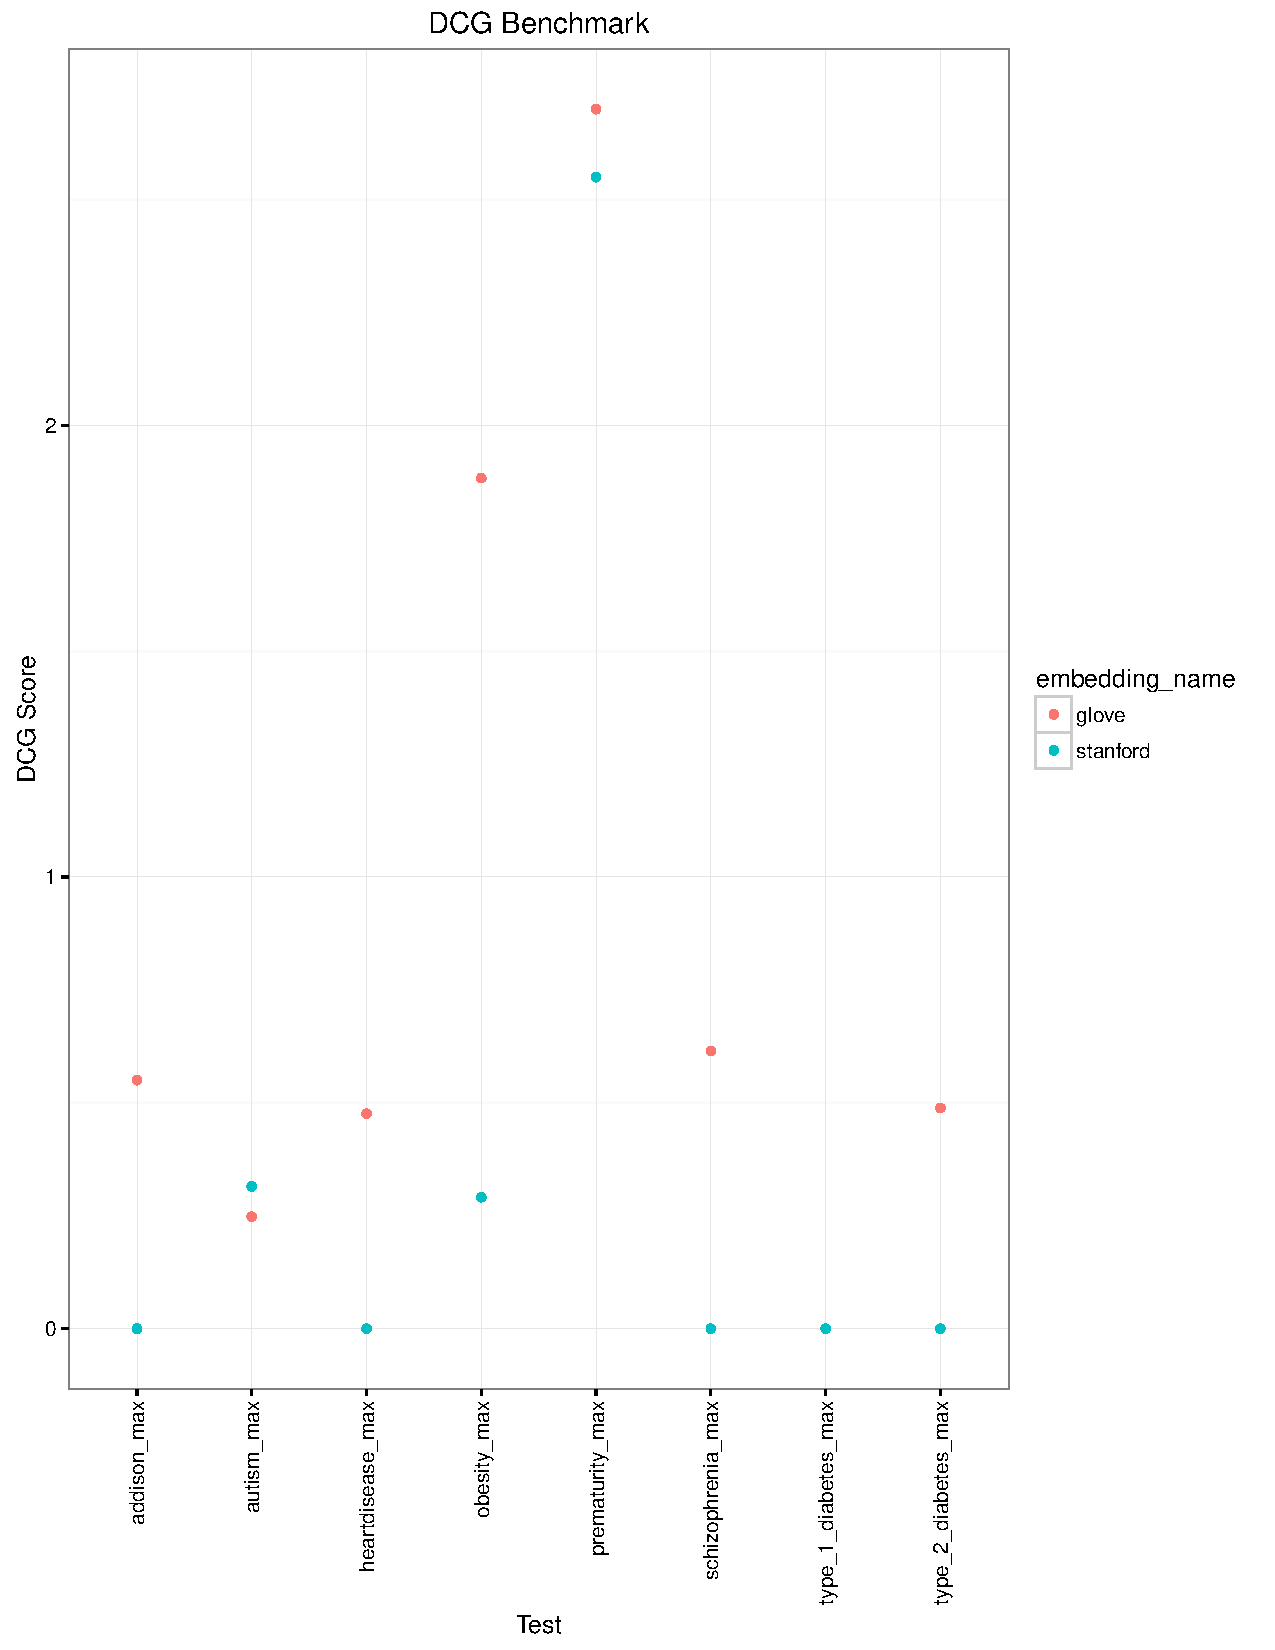
\includegraphics[width=\textwidth]{dcg_plot.pdf}
        \caption{DCG}
    \end{subfigure}
    ~ 
    \begin{subfigure}[b]{0.5\textwidth}
        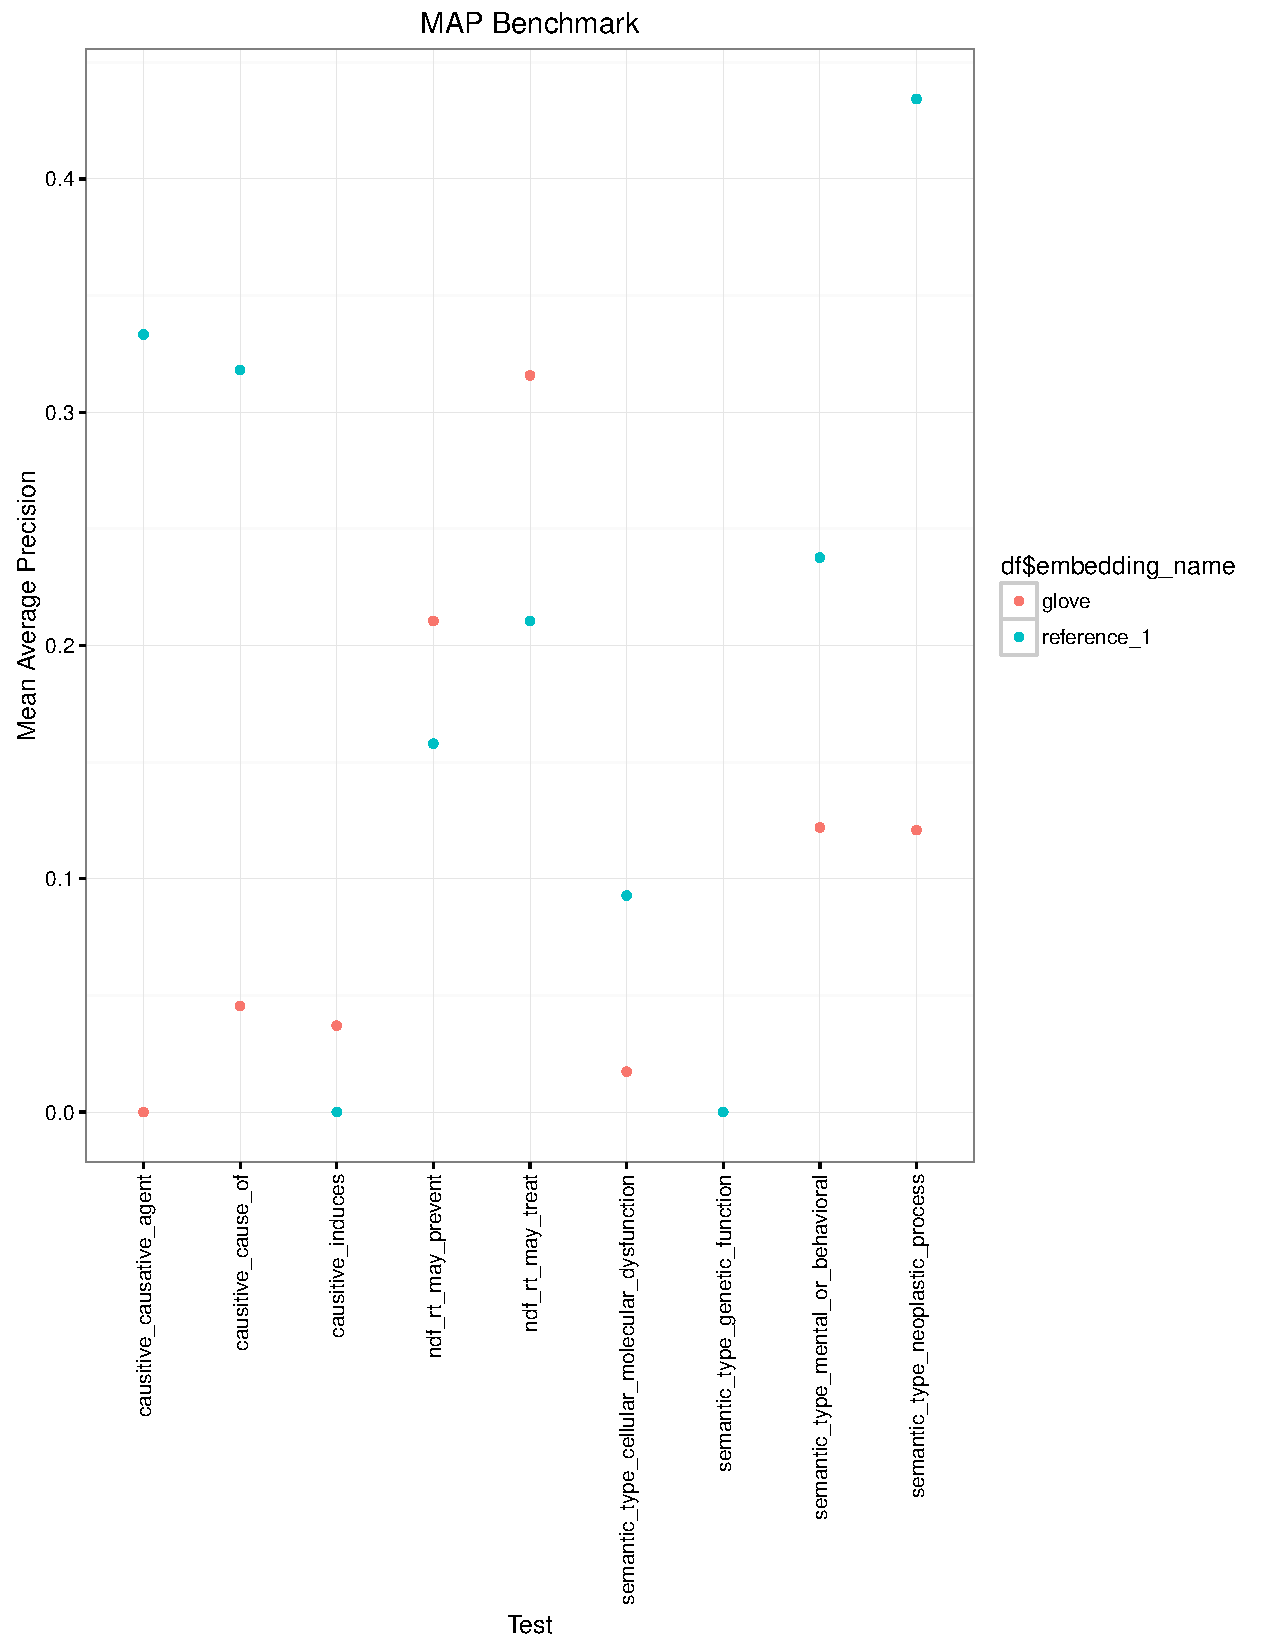
\includegraphics[width=\textwidth]{map_plot.pdf}
        \caption{MAP}
    \end{subfigure}
}
    \caption{Comparison of Stanford and Glove}
\end{figure}

\bibliographystyle{ws-procs11x85}Command \captionbox already defined.
\bibliography{ws-pro-sample}

\end{document}
